\documentclass[tikz,border=8pt]{standalone}

\usepackage[T1]{fontenc}
\usepackage{helvet}
\usepackage{amsmath,amssymb}
\renewcommand{\familydefault}{\sfdefault}
\usetikzlibrary{arrows.meta,calc}

\definecolor{ink}{HTML}{243347}
\definecolor{muted}{HTML}{65758A}
\definecolor{line}{HTML}{D8E1EA}
\definecolor{wash}{HTML}{F5F8FB}
\definecolor{srblue}{HTML}{2673C9}
\definecolor{qcdorange}{HTML}{C66B23}
\definecolor{crviolet}{HTML}{7955B3}
\definecolor{crteal}{HTML}{168C88}
\definecolor{crrose}{HTML}{B44D7A}

\tikzset{
  card/.style={
    draw=line,fill=white,rounded corners=6pt,line width=0.7pt,
    minimum width=3.35cm,minimum height=3.35cm,inner sep=0pt
  },
  heading/.style={font=\bfseries\fontsize{11}{13}\selectfont,align=center},
  object/.style={font=\fontsize{12}{14}\selectfont,align=center,text=ink},
  cuts/.style={font=\fontsize{10.5}{16}\selectfont,align=center,text=ink},
  connector/.style={draw=line!70!muted,line width=0.8pt},
  arrow/.style={connector,-{Latex[length=1.8mm,width=1.3mm]}}
}

\begin{document}
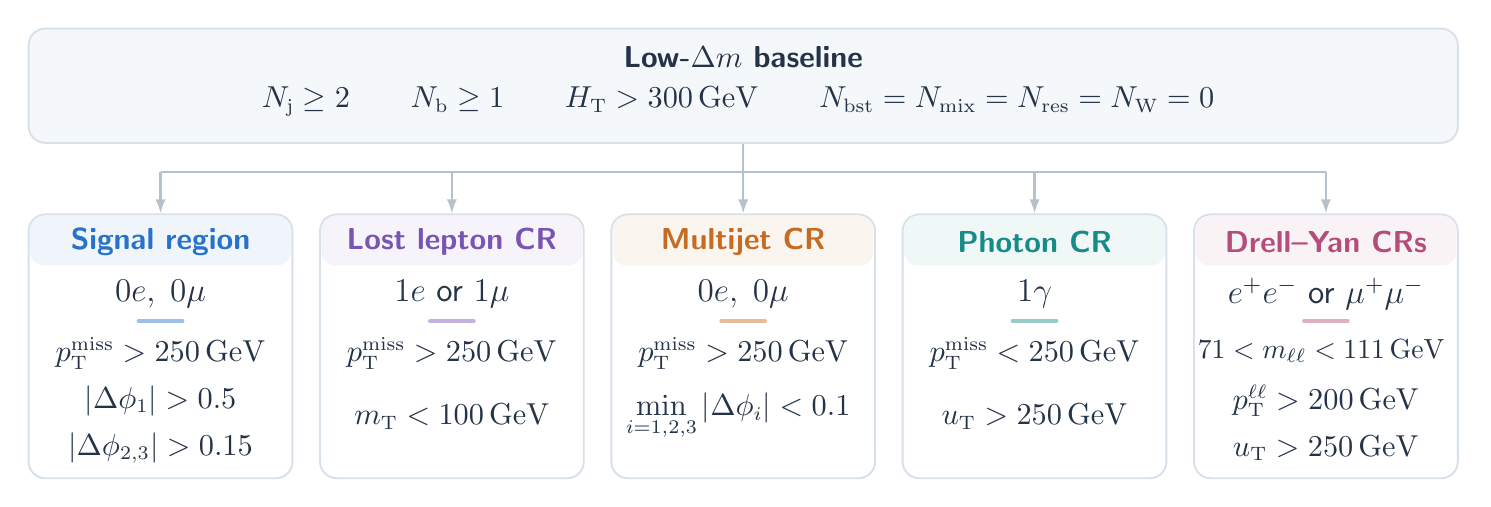
\begin{tikzpicture}[x=1cm,y=1cm,text=ink]

% The complete region definitions are in the adjacent selection table.
\node[draw=line,fill=wash,rounded corners=6pt,line width=0.7pt,
      minimum width=18.15cm,minimum height=1.45cm,inner sep=0pt]
      (baseline) at (7.4,5.28) {};
\node[heading,text=ink] at (7.4,5.65) {Low-$\Delta m$ baseline};
\node[cuts] at (7.4,5.08) {
  $N_{\mathrm{j}}\geq2\qquad N_{\mathrm{b}}\geq1\qquad
   H_{\mathrm{T}}>300\,\mathrm{GeV}\qquad
   N_{\mathrm{bst}}=N_{\mathrm{mix}}=N_{\mathrm{res}}=N_{\mathrm{W}}=0$
};

\draw[connector] (baseline.south) -- (7.4,4.18);
\draw[connector] (0,4.18) -- (14.8,4.18);

\foreach \x/\name/\accent/\title in {
  0/sr/srblue/Signal region,
  3.7/ll/crviolet/Lost lepton CR,
  7.4/qcd/qcdorange/Multijet CR,
  11.1/photon/crteal/Photon CR,
  14.8/dy/crrose/Drell--Yan CRs} {
  \node[card] (\name) at (\x,1.97) {};
  \draw[arrow] (\x,4.18) -- (\name.north);
  \fill[\accent!7,rounded corners=5pt]
    ($(\name.north west)+(0.03,-0.03)$)
    rectangle ($(\name.north east)+(-0.03,-0.66)$);
  \node[heading,text=\accent] at (\x,3.30) {\title};
  \draw[\accent!45,line width=1.3pt,line cap=round]
    (\x-0.28,2.29) -- (\x+0.28,2.29);
}

\node[object] at (0,2.64) {$0e,\;0\mu$};
\node[object] at (3.7,2.64) {$1e\ \text{or}\ 1\mu$};
\node[object] at (7.4,2.64) {$0e,\;0\mu$};
\node[object] at (11.1,2.64) {$1\gamma$};
\node[object] at (14.8,2.64) {$e^+e^-\ \text{or}\ \mu^+\mu^-$};

\foreach \x in {0,3.7,7.4} {
  \node[cuts] at (\x,1.88) {$p_{\mathrm{T}}^{\mathrm{miss}}>250\,\mathrm{GeV}$};
}
\node[cuts] at (0,1.28) {$|\Delta\phi_1|>0.5$};
\node[cuts] at (0,0.68) {$|\Delta\phi_{2,3}|>0.15$};
\node[cuts] at (7.4,1.08) {
  $\displaystyle\min_{i=1,2,3}|\Delta\phi_i|<0.1$
};
\node[cuts] at (3.7,1.08) {$m_{\mathrm{T}}<100\,\mathrm{GeV}$};
\node[cuts] at (11.1,1.88) {$p_{\mathrm{T}}^{\mathrm{miss}}<250\,\mathrm{GeV}$};
\node[cuts] at (11.1,1.08) {$u_{\mathrm{T}}>250\,\mathrm{GeV}$};
\node[cuts,font=\fontsize{10}{14}\selectfont] at (14.8,1.91) {
  $71<m_{\ell\ell}<111\,\mathrm{GeV}$
};
\node[cuts] at (14.8,1.28) {$p_{\mathrm{T}}^{\ell\ell}>200\,\mathrm{GeV}$};
\node[cuts] at (14.8,0.68) {$u_{\mathrm{T}}>250\,\mathrm{GeV}$};

\end{tikzpicture}
\end{document}
